\section{System Details}
As already mentioned in System Overview section, the BPM system consists of three components. Of the three components, the client Android application plays the most important role in our system. This section of the paper will elaborate on the client Android application component in more detail. First of all, we will discuss the interaction between the client Android application and the application server focusing on retrieving the MAC address and PIN of the parking lot Bluetooth device. Then we will discuss how the client Android application uses the MAC address and PIN to scan the correct device and initiating a connection establishment between the client smartphone and the parking lot Bluetooth device.

\subsection{Purchasing Parking Permit}
In order to use BPM system, the user must register with our system and purchase the parking permit through the client Android application. Parking permit purchasing process starts with searching for a parking lot. As shown in Figure \ref{fig:searching}, parking lots can be easily searched by ZIP code, which shows a list of available parking lots in the region.

\begin{figure}[ht]
	\centering
		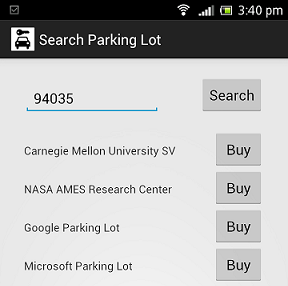
\includegraphics[width=3in]{figure/sys_detail_search.png}
		\caption{The client Android application allows users to easily search parking lots by ZIP code}
	\label{fig:searching}
\end{figure}

When the user purchases the parking permit, the application makes an HTTP POST request to the server requesting that the user wants to purchase a permit of a parking lot with the specific parking lot ID. Then the server replies back to the client with the MAC address of the Bluetooth device and the PIN associated with the Bluetooth device (as shown in Figure \ref{fig:mac_pin}).

\begin{figure}[ht]
	\centering
		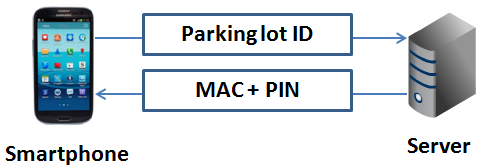
\includegraphics[width=3in]{figure/sys_detail_permit.png}
		\caption{The application requests a permit with a parking lot ID, and the server responses with MAC address and PIN}
	\label{fig:mac_pin}
\end{figure}

Once the client application receives the MAC and PIN, it starts scanning for available Bluetooth devices, and establishes a communication channel if the found Bluetooth device's MAC address matches with the MAC address of the permit the user has purchased. Once the connection is established, the client is ready to control the parking lot gate.

\subsection{Controlling Parking Lot Gate}
Using Bluetooth technology allows users to control the parking lot gate with minimum user effort compared to the current system of using RFID access card or paper tickets. However, this approach is not a perfect solution, and therefore has some drawbacks as well. The range of Bluetooth signal is quite long that it may trigger the connection establishment and open the gate while the authorized vehicle is not even close to the gate. It enables unauthorized vehicles to piggy back the parking lot access, if they are in front of authorized vehicle users. 

\begin{figure}[ht]
	\centering
		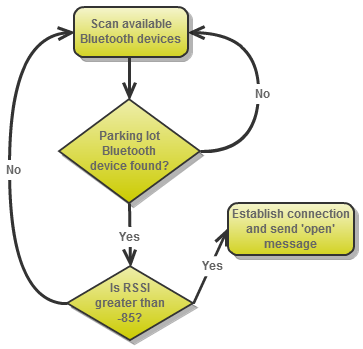
\includegraphics[width=3in]{figure/sys_detail_flow_chart.png}
		\caption{RSSI of the Bluetooth device is checked during the parking lot gate control process to ensure that the authorized user is in front of the gate}
	\label{fig:flowchart}
\end{figure}

In order to address this particular issue, we have conducted a number of experiments to determine the position of the authorized user's vehicle. We have collected the Radio Signal Strengthh Indicator (RSSI) of the Bluetooth device at various location. The experiment has shown that various location of the user's vehicle results in different range of the RSSIs of Bluetooth device. By setting appropriate threshold of RSSI and only initiating the connection establishment above the threshold, we could mostly eliminate the problem of granting unauthorized users access to the parking lot. Figure \ref{fig:flowchart} shows the flow of parking lot gate control process.